\documentclass[11pt, a4paper, twoside]{article}
% font size could be 10pt (default), 11pt or 12 pt
% paper size coulde be letterpaper (default), legalpaper, executivepaper,
% a4paper, a5paper or b5paper
% side coulde be oneside (default) or twoside 
% columns coulde be onecolumn (default) or twocolumn
% graphics coulde be final (default) or draft 
%
% titlepage coulde be notitlepage (default) or titlepage which 
% makes an extra page for title 
% 
% paper alignment coulde be portrait (default) or landscape 
%
% equations coulde be 
%   default number of the equation on the rigth and equation centered 
%   leqno number on the left and equation centered 
%   fleqn number on the rigth and  equation on the left side
%	

\usepackage{graphicx}


\title{A not so small \LaTeX{} Article Template}
\author{Your Name\thanks{Corresponding Author}  \\
	    Your University\\ Email:  \\
	\and 
	The Other Dude \\
	Your University\\ Email: \\
	}

\date{} 
% \date{\today} date coulde be today 
% \date{25.12.00} or be a certain date
% \date{ } or there is no date 
\begin{document}
% Hint: \title{what ever}, \author{who care} and \date{when ever} could stand 
% before or after the \begin{document} command 
% BUT the \maketitle command MUST come AFTER the \begin{document} command! 
\maketitle


\begin{abstract}
Short introduction to subject of the paper \ldots 
\end{abstract}

%\tableofcontents % create a table of contens 



\section{Introduction}
Make it possible for all to write documents with \LaTeX{}!

This document is an example of \texttt{thebibliography} environment using 
in bibliography management. Three items are cited: \textit{The \LaTeX\ Companion} 
book \cite{latexcompanion}, the Einstein journal paper \cite{einstein}, and the 
Donald Knuth's website \cite{knuthwebsite}. The \LaTeX\ related items are
\cite{latexcompanion,knuthwebsite}. 

\subsection{more introduction}
Go more in detail \ldots

\subsubsection{even more introduction}
come to the point \ldots

\paragraph{Paragraphs}
A paragraph is small but 

\subparagraph{Subparagraphs}
subparagraphs are smaller! 

\paragraph{Outline}
First we start with a little example of the article class, which is an 
important documentclass. But there would be other documentclasses like 
book \ref{book}, report \ref{report} and letter \ref{letter} which are 
described in Section \ref{documentclasses}. Finally, Section 
\ref{conclusions} gives the conclusions.



\section{Documentclasses} \label{documentclasses}

\begin{itemize}
\item article
\item book 
\item report 
\item letter 
\end{itemize}


\begin{enumerate}
\item article
\item book 
\item report 
\item letter 
\end{enumerate}

\begin{description}
\item[article\label{article}]{Article is \ldots}
\item[book\label{book}]{The book class \ldots}
\item[report\label{report}]{Report gives you \ldots}
\item[letter\label{letter}]{If you want to write a letter.}
\end{description}

\section{Some Math}
Math in text is called in line math just put \$ character around 
the math think. Like $ a^2 + b^2 = c^2 $. It looks better if you use 
this 
\[a^2 + b^2 = c^2\]


\section{Tabular and Figures}
No paper without a tabular. See the Table \ref{tab:template}

\begin{table}[!b]
\centering
\begin{tabular}{|l|c|c|c|c|c|}
\hline
Product & 1 & 2 & 3 & 4 & 5\\
\hline
Price & 124.- & 136.- & 85.- & 156.- & 23.-\\
Guarantee [years] & 1 & 2 & - & 3 & 1\\
Rating & 89\% & 84\% & 51\% & & 45\%\\
\hline
\hline
Recommended & yes & yes & no & no & no\\
\hline
\end{tabular}
\caption{This is a table template}
\label{tab:template}
\end{table}


Fig. \ref{fig1} is the universe.

\begin{figure}
  \caption{A picture of a gull.}
  \centering
    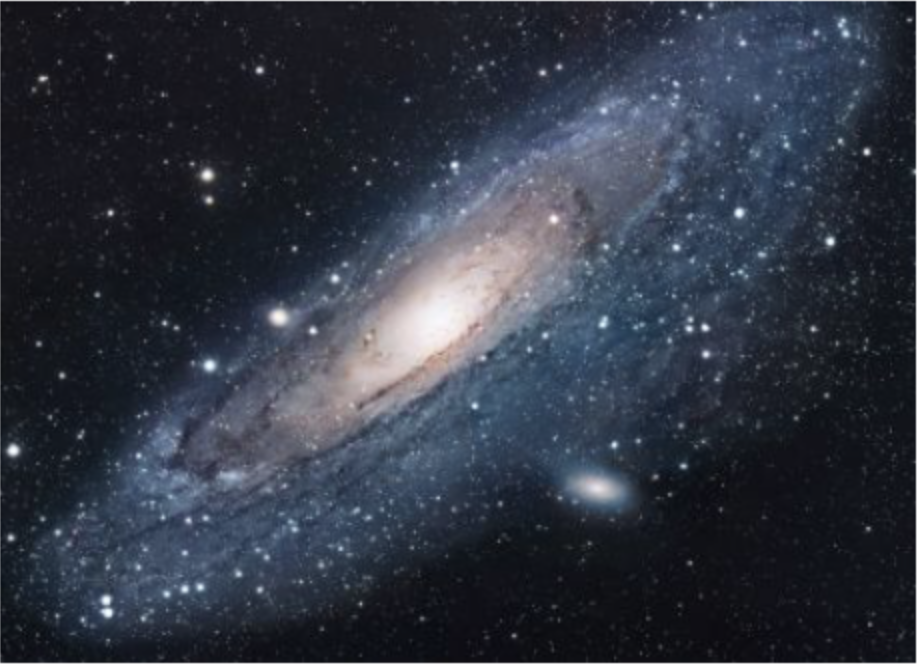
\includegraphics[width=0.5\textwidth]{universe}
  \label{fig1}
\end{figure}


\section{Conclusions}\label{conclusions}
There is no longer \LaTeX{} example which was written by \cite{knuthwebsite}.

\begin{thebibliography}{9}
\bibitem{latexcompanion} 
Michel Goossens, Frank Mittelbach, and Alexander Samarin. 
\textit{The \LaTeX\ Companion}. 
Addison-Wesley, Reading, Massachusetts, 1993.

\bibitem{einstein} 
Albert Einstein. 
\textit{Zur Elektrodynamik bewegter K{\"o}rper}. (German) 
[\textit{On the electrodynamics of moving bodies}]. 
Annalen der Physik, 322(10):891-921, 1905.

\bibitem{knuthwebsite} 
Knuth: Computers and Typesetting,
\\\texttt{http://www-cs-faculty.stanford.edu/\~{}uno/abcde.html}
\end{thebibliography}

\end{document}
